% Revision build: line-numbered single-column manuscript with the
% reviewer responses appended. The Makefile splits the resulting PDF
% into the revised manuscript (line-numbered) and the response
% document (no line numbers, page numbers reset to 1) using the page
% number written to review-responses-pagenum.txt by the response block
% at the end of this file.
%
% The original bioinfo.cls build (main.tex) is untouched and remains
% the canonical typeset version for final submission.

\documentclass[11pt]{article}
\usepackage[margin=1in]{geometry}
\usepackage[T1]{fontenc}
\usepackage{amsmath}
\usepackage{amssymb}
\usepackage[round]{natbib}
\usepackage{fancyhdr}
\usepackage{xcolor}
\usepackage{lineno}

% Review response macros and \revpoint / \revref / \llabel commands.
% Loaded before paper/header so the real definitions win over the
% \providecommand no-ops in the shared header.
\input{review-response-commands}

% Packages
\let\href\undefined
\usepackage[hidelinks]{hyperref}
\usepackage[capitalize]{cleveref}
\usepackage{xspace}
\usepackage{amsmath}
\usepackage{booktabs}
\usepackage{graphicx}

% Remove section numbering
\setcounter{secnumdepth}{0}

% Commands
\newcommand{\mkado}{\mbox{\texttt{MKado}}\xspace}

% No-op fallbacks for review-response back-link macros. main_revision.tex
% loads review-response-commands.tex (which provides the real \revpoint /
% \llabel via \linelabel) before this header is read, so these
% \providecommand calls are skipped there. preprint.tex and main.tex do
% not load review-response-commands, so they fall through to these no-ops
% and the manuscript still compiles cleanly.
\providecommand{\revpoint}[2]{}
\providecommand{\llabel}[1]{}

\newcommand{\beginsupplement}{%
    \setcounter{table}{0}
    \renewcommand{\thetable}{S\arabic{table}}%
    \setcounter{figure}{0}
    \renewcommand{\thefigure}{S\arabic{figure}}%
    \renewcommand{\theHtable}{supp.\arabic{table}}%
    \renewcommand{\theHfigure}{supp.\arabic{figure}}%
}


\pagestyle{fancy}
\setlength{\headheight}{14.5pt}
\fancyhead[L]{}
\fancyhead[R]{\textbf{MKado: McDonald-Kreitman test toolkit}}

% Stub out bioinfo.cls commands so paper/abstract.tex etc compile under
% article class.
\newcommand{\subtitle}[1]{\begin{center}\large #1\end{center}}
\newcommand{\corresp}[1]{}
\newcommand{\history}[1]{}
\newcommand{\editor}[1]{}
\newcommand{\firstpage}[1]{}
\renewcommand{\abstract}[1]{%
  \begin{center}\textbf{Abstract}\end{center}
  \begin{quote}\small #1\end{quote}
  \medskip}

\begin{document}

\linenumbers

\title{MKado: a toolkit for McDonald-Kreitman tests of natural selection}
\author{Angel G.\ Rivera-Col\'{o}n\textsuperscript{1},
  Clara T.\ Rehmann\textsuperscript{1},
  and Andrew D.\ Kern\textsuperscript{1,*}\\[4pt]
  \small\textsuperscript{1}Institute of Ecology and Evolution and Department of Biology,
  University of Oregon, Eugene, OR 97403, USA\\
  \small\textsuperscript{*}Correspondence: \href{mailto:adkern@uoregon.edu}{adkern@uoregon.edu}}
\date{}

\maketitle

\input{paper/abstract}

\input{paper/introduction}
\section{Features and Implementation}

\mkado is implemented in Python
and provides both a command-line interface built on
\texttt{Typer} and a Python API for programmatic use.
It accepts codon-aligned FASTA files as input,
requiring no pre-processing or external format conversion.
Sequences are automatically partitioned into ingroup and outgroup sets
by name pattern matching,
supporting both multi-species alignments in a single FASTA file
and separate files containing ingroup or outgroup sequences.
\revpoint{1}{1}\revpoint{2}{2}\mkado{} also accepts variant-call
input via the \texttt{vcf} subcommand, which takes a multi-sample
ingroup VCF, a single-sample outgroup VCF, a reference FASTA, and a
GFF3 annotation, derives codon-level polymorphism and divergence
counts directly, and supports the full set of MK analyses available
to the FASTA workflow. Together, these two input modes distinguish
\mkado{} from FASTA-only tools (\texttt{DnaSP}, \texttt{asymptoticMK})
and from VCF-only tools (\texttt{degenotate}, \texttt{fastDFE}).
Full documentation, including tutorials and API reference,
is available at \url{https://mkado.readthedocs.io}.

\paragraph{Analysis methods}
\mkado implements five MK-based analyses.
The \textit{standard} test computes the classical $2 \times 2$ table
of nonsynonymous and synonymous changes
in polymorphism and divergence,
with significance assessed by Fisher's exact test
or the $G$-test.
\revpoint{2}{1}$D_n$ and $D_s$ are the numbers of fixed differences
between ingroup and outgroup at codon positions where the inferred
substitution is nonsynonymous or synonymous, respectively, under the
supplied genetic code.
$P_n$ and $P_s$ are the corresponding numbers of ingroup
polymorphic sites at which the derived (non-outgroup) allele
segregates above an optional frequency threshold
(default zero, i.e.\ all polymorphisms;
\texttt{-{}-min-freq~$X$} excludes sites with derived allele
frequency below $X$, and \texttt{-{}-no-singletons} excludes
singletons by setting the threshold to $1/n$ for sample size $n$).
By default $P_n$ and $P_s$ follow the \texttt{DnaSP} convention
and exclude sites that also segregate in the outgroup;
\texttt{-{}-pool-polymorphisms} pools ingroup and outgroup
polymorphism instead.
Summary statistics include the neutrality index \citep[NI;][]{rand1996},
$\alpha$ \citep{smith2002},
and the Direction of Selection statistic
\citep[DoS;][]{stoletzki2011}.
\revpoint{1}{2}Tests that depend on derived allele frequency---the
asymptotic and imputed MK tests described below---require knowing the
derived allele at each polymorphic site. \mkado{} polarizes alleles
automatically using the outgroup: at each polymorphic site, the
allele matching the outgroup is treated as ancestral and any
non-outgroup allele as derived. This automatic single-outgroup
polarization is distinct from the \textit{polarized} MK test below,
which uses a \emph{second} outgroup to attribute each fixed
difference to either the ingroup or the outgroup lineage.
The \textit{polarized} test uses a second outgroup
to infer the ancestral state at each fixed difference,
assigning divergence to the ingroup or outgroup lineage
for lineage-specific inference.
The \textit{asymptotic} test bins polymorphisms
by derived allele frequency,
computes $\alpha$ within each bin,
and fits an exponential model $\alpha(x) = a + b e^{-cx}$
to extrapolate the asymptotic $\alpha$ at $x = 1$,
correcting for the contribution of weakly deleterious variants
\citep{messer2013}.
A linear model is also fitted
and AIC selects the better specification,
following \citet{haller2017}.
\revpoint{1}{4}\mkado{} supports both the original per-bin SFS construction of
\citet{messer2013}, in which $P_n(x)$ and $P_s(x)$ count
polymorphic sites with derived allele frequency \emph{equal to}~$x$,
and the cumulative inclusive variant of \citet{uricchio2019}, in
which $P_n(x)$ and $P_s(x)$ count polymorphic sites with derived
allele frequency \emph{at or above}~$x$ (selectable with
\texttt{-{}-sfs-mode \{at,above\}}); the cumulative form has the
same asymptote at $x = 1$ but is more robust to bin-count sparsity
in large samples.
The asymptotic test supports both per-gene
and aggregated (pooled across genes) modes; for the aggregated
mode, two confidence-interval methods are available
(\texttt{-{}-ci-method}): a parametric Monte-Carlo procedure that
samples the curve-fit covariance matrix (default; fast) and a
case-resampling bootstrap that resamples the pooled polymorphism
list and refits per replicate (slower per replicate but more
principled when per-bin counts are small).
The \textit{imputed} test corrects for weakly deleterious mutations
by estimating their contribution from the ratio
of low- to high-frequency synonymous polymorphisms
\citep{murga-moreno2022}.
Polymorphisms are split at a derived allele frequency % Alternatively, change to DAF here
cutoff (default 15\%),
and the expected number of weakly deleterious nonsynonymous
polymorphisms below the cutoff is imputed as
$P_{wd} = P_{n,\text{low}} - P_{n,\text{high}} \times
(P_{s,\text{low}} / P_{s,\text{high}})$.
The corrected count $P_{n}^{*} = P_n - P_{wd}$
is then used in the standard $2 \times 2$ test
to obtain a bias-corrected $\alpha$.
This approach retains more data than simple frequency filtering
while still removing the downward bias from slightly deleterious
variants.
Finally, the Tarone-Greenland $\alpha_\text{TG}$ estimator
\citep{stoletzki2011}
provides an unbiased multi-gene estimate of $\alpha$
by weighting each gene inversely by $P_s + D_s$,
correcting for sample size heterogeneity across loci.

\paragraph{Codon change classification}
When comparing codons that differ at multiple positions,
the assignment of changes as synonymous or nonsynonymous
is not straightforward
because the order of substitutions is unknown.
\mkado pre-computes all shortest mutational paths
between every pair of codons
and weights the synonymous and nonsynonymous contributions
equally across paths,
following the approach of \citet{nei1986}.

\paragraph{Batch processing and output}
MKado's \texttt{batch} command processes directories of alignment files
in parallel using Python's multiprocessing facilities
with configurable worker counts.
Benjamini-Hochberg false discovery rate (FDR) $q$-values
are computed automatically across all genes.
Results are available in human-readable, TSV, or JSON formats.
A companion \texttt{info} command reports alignment diagnostics
(sequence count, length, and codon structure)
for input validation.

To evaluate scaling performance,
we benchmarked \mkado on 12,437 human protein-coding genes
aligned with chimpanzee and orangutan orthologs
from \texttt{OrthoMaM} \citep{orthomam2024},
with polymorphism data from 178 Yoruba individuals
in the 1000 Genomes Project \citep{1000genomes2015}.
Processing all genes with 128 worker threads
completed in 28 seconds, a $\sim$50$\times$ speedup over
single-threaded execution.\revpoint{2}{10} Per-gene work
(alignment parsing, codon classification, and the per-gene MK
computation) takes only milliseconds, so the per-process spawn
overhead from Python's \texttt{multiprocessing} grows
non-negligible relative to per-task work as the worker count
rises. \Cref{fig:benchmark} shows approximately linear scaling
up to roughly 16 workers, with progressively diminishing
efficiency past 32 workers; we therefore recommend setting the
worker count well below the gene count for batch runs at any
scale. For workloads dominated by aggregated tests (asymptotic
MK with case-resampling bootstrap CIs), where per-task work is
much larger, scaling extends usefully to higher worker counts
(\cref{fig:aggregated_runtime}).

\paragraph{Visualization}
\mkado generates publication-ready plots
directly from the command line.
Volcano plots display $-\log_{10}(\text{NI})$
against $-\log_{10}(p)$ for each gene,
with Bonferroni and nominal significance thresholds
(left panel of \cref{fig:volcano}).
The asymptotic test produces $\alpha(x)$ curves
showing the fitted model and bootstrap confidence intervals
(right panel of \cref{fig:volcano}).

\begin{figure*}[!t]
  \centering
  \includegraphics[width=0.48\textwidth]{figures/mk_volcano_pongo.png}\hfill
  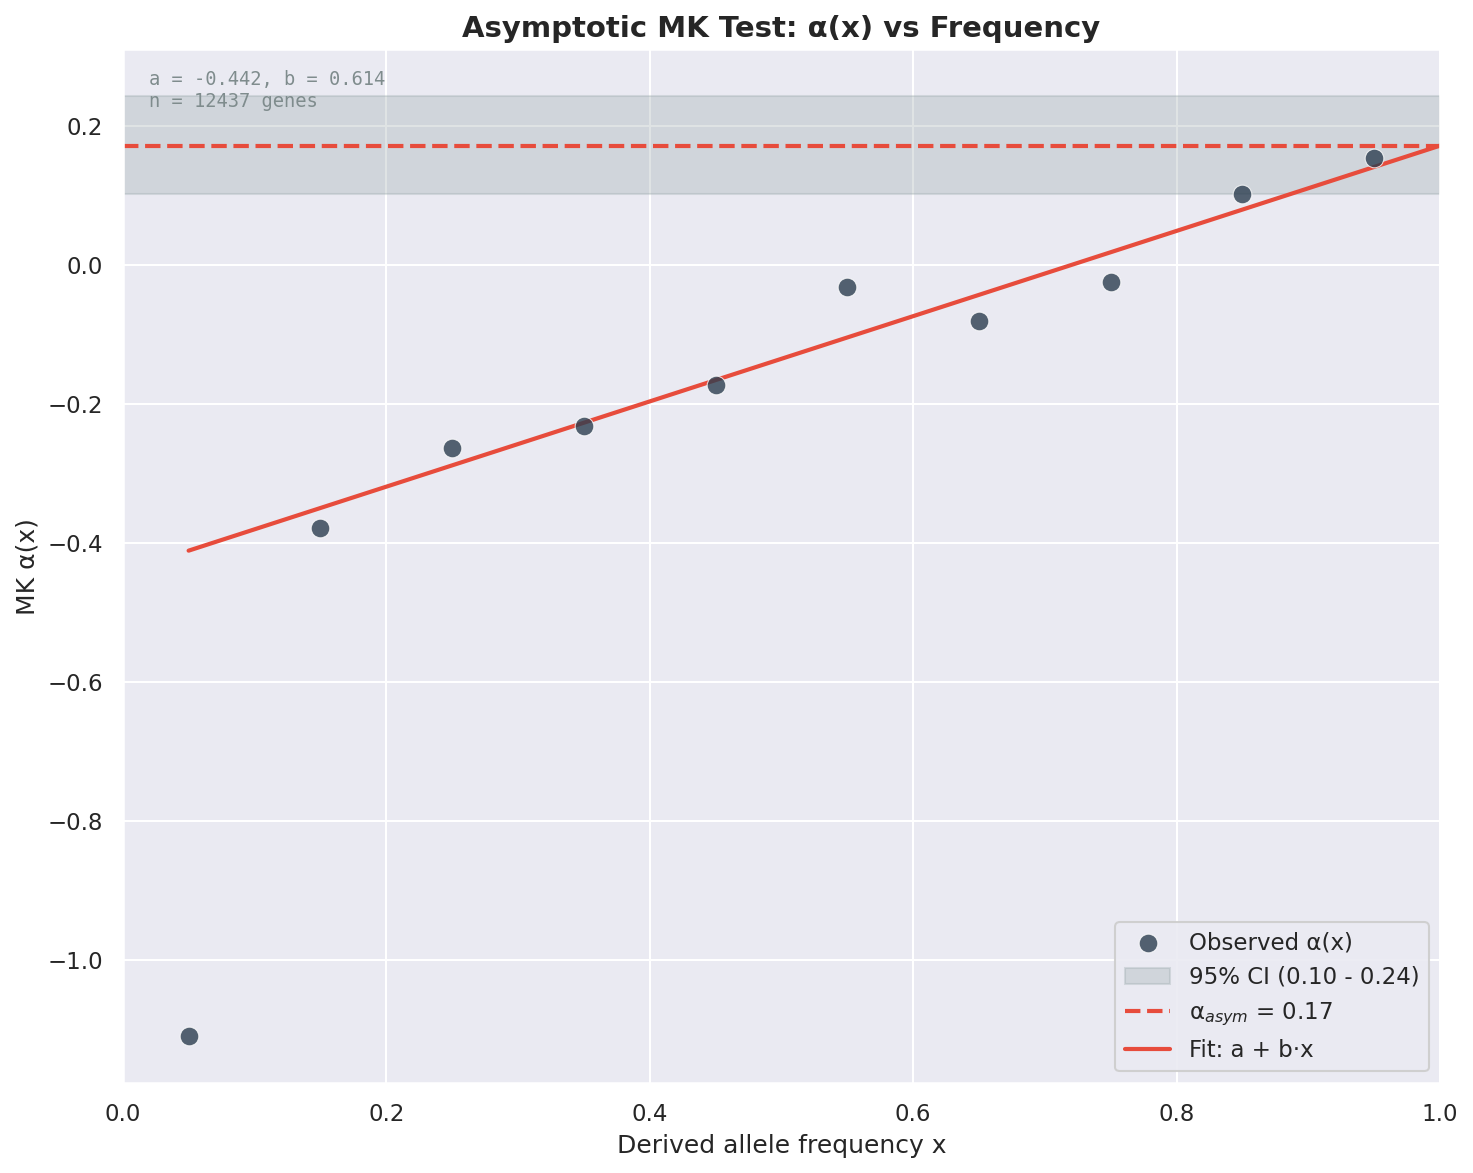
\includegraphics[width=0.48\textwidth]{figures/asymp-OH.png}
  \caption{MK test results for 12,437 human protein-coding genes using
    \textit{Pongo abelii} as the outgroup for divergence.
    % We don't have A or B in the figure above, so changing to left and right
    Left: Volcano plot from per-gene standard MK tests.
    Red points are significant after Bonferroni correction, while
    orange points are nominally significant ($p < 0.05$).
    The dashed lines indicate Bonferroni and nominal thresholds.
    The leftward shift of the cloud (NI $> 1$) reflects the
    well-known excess of weakly deleterious nonsynonymous polymorphism
    in humans.
    Right: Asymptotic $\alpha$ curve for pooled data.
    Points represent the observed $\alpha$ at each derived allele
    frequency cutoff; the solid line represents the fitted curve,
    in this case the linear model selected by AIC. The shaded area
    indicates the 95\% confidence interval around the fitted
    asymptotic $\alpha$ value.}
  \label{fig:volcano}
\end{figure*}

\section{Application}

To demonstrate \mkado at genome scales,
we assembled a dataset of 12,437 human protein-coding genes
with both polymorphism and divergence data.
Codon-aligned orthologous sequences
for human (\textit{Homo sapiens}),
chimpanzee (\textit{Pan troglodytes}),
and orangutan (\textit{Pongo abelii})
were obtained from \texttt{OrthoMaM} v12 \citep{orthomam2024},
which provides one canonical coding-sequence ortholog per gene
across mammalian taxa.
Human intraspecific polymorphism was drawn from 178 Yoruba (YRI)
individuals in the 1000 Genomes Project NYGC high-coverage dataset
\citep{1000genomes2015},
yielding 356 phased haplotypes per gene.

\revpoint{1}{7}For each gene, polymorphism was projected onto the
\texttt{OrthoMaM} alignment in five steps:
(i)~the canonical Ensembl CDS for the gene was reconstructed from
the GRCh38 reference and the GTF-derived exon set, providing the
mapping from CDS position to genomic coordinate;
(ii)~the ungapped human row of the \texttt{OrthoMaM} alignment was
matched against the Ensembl CDS to obtain the alignment-column to
CDS-position correspondence (genes for which this match failed,
typically because of curation differences between
\texttt{OrthoMaM} and Ensembl, were dropped);
(iii)~for every CDS position that survived this match, the
overlapping YRI variants were extracted from the 1000 Genomes
NYGC VCF, with reference-allele identity confirmed and
minus-strand alleles complemented to match the CDS orientation;
(iv)~per-individual phased haplotypes were assembled from the
extracted variants, yielding 356 human haplotype sequences over
the Ensembl CDS positions retained by \texttt{OrthoMaM}; and
(v)~these haplotypes were re-gapped to the \texttt{OrthoMaM}
alignment, dropping any human-CDS columns absent from the
\texttt{OrthoMaM} alignment and inserting the alignment's
existing gap structure (so insertions, deletions, and
non-aligned regions in the multi-species alignment are
preserved). Chimpanzee and orangutan sequences were taken
directly from the \texttt{OrthoMaM} alignment. Multi-transcript
genes are reduced to the single canonical CDS chosen by the
\texttt{OrthoMaM} curation; alternative transcripts are not
analysed separately. The resulting per-gene multi-species FASTAs
are codon-aligned and ready for direct input to \mkado.

Using orangutan as the outgroup,
genome-wide pooled counts were
$D_n$\,=\,94,578, $D_s$\,=\,188,325, $P_n$\,=\,44,850,
and $P_s$\,=\,47,838.
The per-gene standard MK test identified numerous genes
with significant departures from neutrality,
including genes significant after Bonferroni correction
(volcano plot, left panel of \cref{fig:volcano})\revpoint{2}{3}.
As expected,
the majority of testable genes showed NI~$>$~1,
reflecting the well-characterized excess
of slightly deleterious nonsynonymous polymorphism in humans
\citep{li2008}.
Using chimpanzee as the outgroup yielded fewer fixed differences
($D_n$\,=\,37,120, $D_s$\,=\,65,228), roughly 2.5-fold less than
orangutan (left panel of \cref{fig:chimp_mk}),
and no individual genes survived Bonferroni correction,
consistent with the limited power of single-gene tests
at shorter divergence times.

The Tarone-Greenland weighted estimate \citep{stoletzki2011}
across all genes was strongly negative for both outgroups:
$\hat{\alpha}_\text{TG} = -0.853$
(95\% CI: $-0.888$ to $-0.812$)
for orangutan
and $\hat{\alpha}_\text{TG} = -0.651$
(95\% CI: $-0.682$ to $-0.607$)
for chimpanzee,
with corresponding $\text{NI}_\text{TG}$ values of 1.853 and 1.651.
These negative values confirm the pervasive excess
of weakly deleterious nonsynonymous polymorphism in humans.
Excluding singletons shifted both estimates upward
($\hat{\alpha}_\text{TG} = -0.794$ for orangutan;
$-0.606$ for chimpanzee),
as expected given the enrichment of slightly deleterious
variants at low frequency.
Applying a 15\% derived allele frequency cutoff
\citep{fay2001}
brought both estimates close to zero
($\hat{\alpha}_\text{TG} = -0.091$ for orangutan;
$-0.041$ for chimpanzee),
removing the bulk of low-frequency deleterious variants
but still failing to recover a signal of positive selection.
Similarly, the aggregated imputed MK test \citep{murga-moreno2022},
using a 15\% derived allele frequency cutoff,
estimated $\hat{\alpha} = -0.097$ for orangutan
and $\hat{\alpha} = -0.068$ for chimpanzee,
substantially reducing the downward bias
but likewise not recovering a positive signal of adaptation.

In contrast, the aggregated asymptotic MK test,
which models the frequency dependence of $\alpha$
and extrapolates to fixation \citep{messer2013},
successfully recovered a positive signal of adaptive evolution,
estimating $\hat{\alpha} = 0.163$
(95\% CI: 0.075 to 0.253; right panel of \cref{fig:volcano})
using orangutan as the outgroup,
indicating that approximately 16\% of amino acid substitutions
on the human lineage were driven by positive selection.
With chimpanzee as the outgroup the estimate widened to
$\hat{\alpha} = 0.075$ (95\% CI: $-1.22$ to $0.11$;
right panel of \cref{fig:chimp_mk}),
illustrating the greater uncertainty
from the shallower divergence, but also indicating 
a potential biological signal of less frequent adaptive evolution
after the human-Pongo split. 
These results are consistent with previous analyses
of human coding sequences \citep{messer2013}.

The entire analysis---standard MK tests,
Tarone-Greenland estimation, asymptotic estimation,
imputed estimation,
and volcano plot generation for all 12,437 genes---completed
in under one minute on a multi-core workstation
using \mkado's parallel batch mode.


\section*{Acknowledgements}
We thank members of the Kern lab for helpful feedback.


\input{paper/funding}

\bibliographystyle{plainnat}
\bibliography{bibliography}

\pagebreak
\beginsupplement
\section*{Supplementary Results}

\begin{figure}[!ht]
  \centering
  \includegraphics[width=\columnwidth]{figures/mkado_benchmark.pdf}
  \caption{Parallel scaling of \mkado batch processing on 12,437 human
    protein-coding genes. (\textbf{A})~Wall-clock time versus worker threads.
    (\textbf{B})~Speedup relative to single-threaded execution, with ideal
    linear scaling shown as a dashed line. (\textbf{C})~Parallel efficiency
    (speedup divided by thread count).}
  \label{fig:benchmark}
\end{figure}


% === Review Responses (extracted to a separate PDF by the Makefile) ===
\clearpage
% Record the absolute page number where responses begin, for PDF splitting.
\newwrite\pageinfo
\immediate\openout\pageinfo=review-responses-pagenum.txt
\immediate\write\pageinfo{\thepage}
\immediate\closeout\pageinfo
\setcounter{page}{1}
\label{review-responses-start}
\nolinenumbers
\pagestyle{plain}

\begin{center}
{\LARGE \textbf{Response to Reviewers}}\\[1em]
{\large MKado: a toolkit for McDonald-Kreitman tests of natural selection}
\end{center}

\vskip 2em

% Cover letter and point-by-point reviewer responses.
% Reviewer text is verbatim from paper_review.txt; \reply{...} blocks
% are scaffolded as TODO placeholders to be filled in during the revision.

\begin{minipage}[b]{2.5in}
  Resubmission Cover Letter \\
  {\it Bioinformatics}
\end{minipage}
\hfill
\begin{minipage}[b]{5.5in}
  Andrew Kern (on behalf of all authors) \\
  \today
\end{minipage}

\vskip 2em

\noindent
{\bf To the Editor(s) -- }

\vskip 1em

We are writing to submit a revised version of our manuscript titled
``MKado: a toolkit for McDonald-Kreitman tests of natural selection''.
We thank the editor and both reviewers for their thoughtful and
constructive comments, which have substantially strengthened the
manuscript and the underlying software package. The most substantive
changes in this revision are: (i) a new aggregated-genes asymptotic-MK
runtime benchmark addressing Reviewer~1, point~5; (ii) implementation of
the Uricchio et al.~(2019) ``above-$x$'' cumulative SFS for the
asymptotic test, addressing Reviewer~1, point~4; (iii) a polyDFE-style
case-resampling bootstrap CI for asymptotic alpha, addressing the second
half of Reviewer~1, point~5; and (iv) prominent VCF-input and
allele-polarization documentation in both manuscript and docs,
addressing Reviewer~1, points~1--2 and Reviewer~2.

In addition to a Response to Reviewers (in which page/line numbers refer
to the revised manuscript file), we provide a marked-up PDF showing the
differences relative to the original submission.

\vskip 2em

\noindent\hspace{4em}
\begin{minipage}{4.5in}
\noindent
{\bf Sincerely,}

\vskip 2em

{\bf
  Andrew Kern (on behalf of all authors)
}\\
\end{minipage}

\vskip 4em

\pagebreak

%%%%%%%%%%%%%%%%%%%%%%%%%%%%%%%%%%%%%%%%%%%%%%%%%%%%%%%%%%%%%%%%%%%%%%%%%
\reviewersection{1}

\begin{itquote}
McDonald and Kreitman (MK) test is one of the most widely used methods
to test for natural selection. Since its original publication, several
studies have proven its potential for detecting positive selection.
Nowadays, we have several extensions that mitigate the main issue of
the MK test: the presence of slightly deleterious mutations. Here, the
authors present a fast, user-friendly, and well-documented software to
automatize MK tests. The software not only includes multiple MK tests
extensions per gene or aggregated datasets, but also data processing,
multiple testing correction, and visualization features. However, I
have a few minor concerns that I hope the authors can address. Most of
them should be straightforward to test or implement.
\end{itquote}

\reply{We thank the reviewer for the positive assessment and for the
detailed, constructive comments. Each point is addressed in turn below;
the substantive items (especially points~4 and~5) drove the
two largest additions in this revision (cumulative-SFS option and a
new aggregated-genes runtime benchmark with bootstrap CIs).}

%---------- R1.1 ----------
\begin{point}{} % 1.1 -- VCF support visible in docs but not in manuscript
As the authors claim, most of the current software is fragmented. Some
tools can deal with VCF or multi-FASTA data (\texttt{degennotate},
\texttt{fastDFE}, \texttt{iMKT}; \url{https://doi.org/10.1093/molbev/msad270},
\url{https://doi.org/10.1093/molbev/msae070},
\url{https://doi.org/10.1093/nar/gkz372}), some have already implemented
several of the MK tests presented here (\texttt{MKtest.jl};
\url{https://doi.org/10.1093/g3journal/jkae031}), others can polarise
alleles (\texttt{fastDFE}; \url{https://doi.org/10.1093/molbev/msae070}).
\mkado unifies it on a user-friendly Python package. The documentation
shows that \mkado can deal with VCF files similarly to \texttt{fastDFE},
but I cannot see this mentioned in the paper. The authors should
include it in the main text, since handling both VCF and multi-FASTA
files is an important feature.
\end{point}

\reply{TODO: describe added VCF paragraph in Features section, new row
in the comparison table, and citations to the named alternatives.}

%---------- R1.2 ----------
\begin{point}{} % 1.2 -- automatic allele polarization vs polarized MK
In addition to describing the Polarised MK Test, the authors should
state in the main text that \mkado uses outgroup sequences to polarize
alleles. As far as I understand, this is done automatically and is
well described in the software documentation. Nonetheless, I would
recommend that the authors clarify the automatic allele polarization
required to run tests such as the asymptotic or imputed MK tests
(where polarization is mandatory or recommended), as distinct from the
polarised MK test, which specifically tests for selection along a
lineage. As I said, this is already well explained in the
documentation, so it should be straightforward to include in the paper
to avoid any misunderstanding.
\end{point}

\reply{TODO: describe new ``Allele polarization'' subsection in Methods.}

%---------- R1.3 ----------
\begin{point}{} % 1.3 -- TG alpha + imputed / FWW combination
When using the Tarone-Greenland Alpha, is the standard MK test
applied? Would it not be beneficial to correct for slightly deleterious
mutations by simply using the imputed or Fay, Wyckoff and Wu frequency
threshold correction?
\end{point}

\reply{TODO: explain that \texttt{--alpha-tg --min-freq X} already
applies the FWW frequency-threshold correction within
$\alpha_\text{TG}$; decline the imputed $\times$ TG combination as an
unvalidated novel estimator.}

%---------- R1.4 ----------
\begin{point}{} % 1.4 -- Uricchio et al. 2019 above-x SFS option
The authors should include an option to modify the SFS as described in
Uricchio et al.\ (2019) (see supplementary material,
\url{https://doi.org/10.1038/s41559-019-0890-6}):

\begin{itquote}
We note that the original asymptotic-MK approach takes $P_N(x)$ and
$P_S(x)$ as the number of polymorphic sites at frequency $x$ rather
than above $x$, but this approach scales poorly as sample size
increases since most common allele frequencies $x$ have very few
polymorphic sites in large samples. We therefore define $P_N(x)$ and
$P_S(x)$ as stated above since these quantities trivially have the
same asymptote but are less affected by changing sample size.
\end{itquote}

The asymptotic estimation would greatly benefit from this modification,
producing more robust results. The authors can follow
\url{https://github.com/jmurga/MKtest.jl/blob/main/src/polymorphism.jl}
to implement it.
\end{point}

\reply{TODO: describe new \texttt{--sfs-mode}\,\{\texttt{at},\texttt{above}\}
flag, default \texttt{at} (Messer \& Petrov 2013) for backward
compatibility, with the cumulative inclusive-tail variant available
under \texttt{above}; cite Uricchio 2019.}

%---------- R1.5 ----------
\begin{point}{} % 1.5 -- runtime benchmarks: composition + aggregated
Do the runtime plots show only the batch processing of the 12,437
human genes, or also the execution of the imputed or standard MK test?
If the tests are not included on runtime, I would recommend that the
authors incorporate both processing and MK test estimation, since this
should not substantially affect the benchmark. Moreover, I'm assuming
the author are not providing runtime benchmark for asymptotic
estimations. Because asymptotic estimation would probably fail at the
gene level or provide unreliable results (as the authors properly
note), I will recommend two approaches:

\begin{itemize}
\item[(i)] Following Murga-Moreno et al.\ (2022)
(\url{https://doi.org/10.1093/g3journal/jkac206}), the authors can
aggregate at least 1{,}000 random genes to ensure reliable estimation
on human data and run the benchmark over a reasonable number of
replicates.
\item[(ii)] They can add the polyDFE bootstrapping strategy to resample
the SFS over the 12{,}437 aggregated genes. This is a common strategy
for obtaining reliable alpha confidence interval (CI) estimates (e.g.,
Castellano et al.\ 2019;
\url{https://doi.org/10.1534/genetics.119.302494}). The authors
currently estimate CI via Monte Carlo, but adding a bootstrap
resampling strategy would benefit both runtime benchmarks and the
reliability of alpha estimates for any MK test provided. See the
\texttt{bootstrapData} function at
\url{https://github.com/paula-tataru/polyDFE/blob/master/postprocessing.R}
or
\url{https://fastdfe.readthedocs.io/en/latest/_modules/fastdfe/spectrum.html#Spectrum.resample}.
\end{itemize}

This way, non-expert users would not face runtimes longer than those
shown in Figure S1. Since the software scaling is nearly perfect,
testing approximately 1{,}000 aggregated datasets should be
informative enough.
\end{point}

\reply{TODO: describe (a) clarified composition of existing benchmarks
(parsing $+$ site counting $+$ test $+$ output), (b) new
aggregated-asymptotic benchmark and supplementary figure built on
the 1{,}000-gene-per-replicate regime
(\texttt{examples/benchmarks/aggregated\_asymptotic\_runtime.py}), and
(c) new \texttt{--ci-method bootstrap} option for asymptotic alpha,
implementing case-resampling refit per replicate.}

%---------- R1.6 ----------
\begin{point}{} % 1.6 -- Ls, Ln; omega_a, omega_na decomposition
Since the authors already manually estimate the shortest mutational
paths and weight synonymous and nonsynonymous sites following Nei and
Gojobori (1986), can they include the total number of synonymous and
nonsynonymous sites ($L_s$, $L_n$)? It should then be straightforward
to also implement $\omega_a$ and $\omega_{na}$, as decomposed in
Coronado-Zamora et al.\ (2019)
(\url{https://academic.oup.com/gbe/article/11/5/1463/5480667}):
\[
\omega_a = \alpha \cdot \omega, \qquad
\omega_{na} = (1 - \alpha) \cdot \omega.
\]
\end{point}

\reply{TODO: describe new \texttt{omega} command computing $L_n$, $L_s$,
$\omega = (D_n / L_n) / (D_s / L_s)$ and the
$\omega_a$ / $\omega_{na}$ decomposition with confidence intervals.}

%---------- R1.7 ----------
\begin{point}{} % 1.7 -- OrthoMaM polymorphism projection writeup
The authors followed an intelligent strategy using the OrthoMaM
database to obtain human $D_n$, $D_s$, $P_n$, and $P_s$ counts. I
think projecting the polymorphic data onto the ortholog alignments
could provide an useful feature when working with non-model species
available within OrthoMaM database. I understand that including such
a feature will be challenging, but a more detailed explanation of the
polymorphism projection procedure would help users working with
non-model organisms.
\end{point}

\reply{TODO: point at new ``Working with ortholog alignments'' section
in the documentation tutorial and a methods paragraph that summarizes
the OrthoMaM coordinate-mapping pipeline (alignment source, VCF
liftover, indel handling, multi-transcript reconciliation). Note that
the standalone \texttt{mkado project} subcommand is deferred to a
future release per the reviewer's allowance.}

%%%%%%%%%%%%%%%%%%%%%%%%%%%%%%%%%%%%%%%%%%%%%%%%%%%%%%%%%%%%%%%%%%%%%%%%%
\reviewersection{2}

\begin{itquote}
This is a concise manuscript reporting a standalone package
specifically designed for computing several flavours of the classical
McDonald-Kreitman test. The length of the manuscript, level of details
and information provided are appropriate. I agree with the authors
that such as tool can be a benefit for the community by filling a gap
in the set of available programs. I would say that \mkado fulfils its
tasks successfully. I had the chance to test the package and I found
it satisfying so my review will be positive. Nevertheless I will seize
this opportunity to provide feedback after looking at the code and
testing the tool.
\end{itquote}

\reply{We thank the reviewer for the positive overall assessment and
for testing the package end-to-end. The detailed, code-level feedback
was particularly valuable; each point is addressed below.}

%---------- R2.1 ----------
\begin{point}{} % 2.1 -- formal definition of Pn and Ps
[The text has a good structure.] However, I would recommend that both
the article and the documentation describe formally the basic
statistics used. There are detailed formulas for variants of the MK
tests, $D_n$ and $D_s$ are clearly defined, but $P_n$ and $P_s$ are
not, actually (or not completely).
\end{point}

\reply{TODO: describe new explicit definitions of $P_n$ and $P_s$ in
the manuscript Methods (with handling of singletons, the
\texttt{--pool-polymorphisms} option, and the derived-allele-frequency
threshold) and the matching tightening of dataclass docstrings in the
package.}

%---------- R2.2 ----------
\begin{point}{} % 2.2 -- VCF support not mentioned in manuscript
I am surprised that the possibility of importing VCF data is not
mentioned in the manuscript. I suppose that this was a recent addition
to the package. This would be an attractive addition to the article.
\end{point}

\reply{TODO: cross-reference response to Reviewer~1, point~1 (added
VCF paragraph and comparison-table row).}

%---------- R2.3 ----------
\begin{point}{} % 2.3 -- Figure 1 caption: two-panel
Figure 1 should be cited slightly differently as it shows both the
volcano plot and the asymptotic MK test display.
\end{point}

\reply{TODO: describe the caption rewrite (left/right panel
description) and the in-text references that no longer mistakenly
refer to a single panel.}

%---------- R2.4 ----------
\begin{point}{} % 2.4 -- __init__.py outdated (version, package name)
The main \texttt{\_\_init\_\_.py} file is outdated as of this writing.
First, the hardcoded version number is still 0.3.0 while the package
has been ported to 0.4.0. Second, the package name in the file
docstring is still ``mikado'', which is the original name of the
project.
\end{point}

\reply{TODO: confirm the version-string and docstring fix in
\texttt{src/mkado/\_\_init\_\_.py} (single-source-of-truth via
\texttt{importlib.metadata.version}).}

%---------- R2.5 ----------
\begin{point}{} % 2.5 -- shell completion options unclear; slow
I noticed that the umbrella command has options to manage shell
completion. They were not clear to me at first sight and it is rather
unexpected to find them as the option of the umbrella command, which
is not expected to do anything. Maybe a ``setup'' command would
clarify it but this is not essential. In any case I recommend adding a
sentence to the help page to explain that these options allow to
configure automatic shell completion. On my system, shell completion
was painfully slow so the feature was doing more harm than good.
\end{point}

\reply{TODO: describe the help-text addition for
\texttt{--install-completion} / \texttt{--show-completion} on the
umbrella command, plus a new ``Shell completion'' subsection in the
docs noting that completion may be slow on some shells and can simply
be left uninstalled.}

%---------- R2.6 ----------
\begin{point}{} % 2.6 -- subcommand-without-args behaviour
When called without argument, the different commands end up with an
error, which is somewhat inconsistent with the behaviour of the
umbrella command (which displays the help page). But it is a perfectly
acceptable behaviour and up to the authors. Commands have logical and
relevant options.
\end{point}

\reply{TODO: short response noting the reviewer's allowance to keep
the existing behaviour, or describe a small CLI tweak that prints help
when a required positional is missing.}

%---------- R2.7 ----------
\begin{point}{} % 2.7 -- output filename specification
The commands write a progress bar and some feedback to the standard
error stream, obviously to enable standard output redirection to
capture the output. Unless I missed it, there is no way to specify
[an] output file name. The choice that has been made is not perfectly
complying with conventions regarding the use of the standard error
stream but it is not unusual either.
\end{point}

\reply{TODO: describe the new \texttt{--output} / \texttt{-o} flag (or
explicitly note that stdout redirection plus the existing
\texttt{--format} flag already covers this case, if we decide not to
add a new flag).}

%---------- R2.8 ----------
\begin{point}{} % 2.8 -- ruff out of user manual; "third outgroup"
The package is adequately documented by a fairly complete README
available on the git and PyPI repositories, and, more in more details
by a readthedocs page. [A] small remark would be that I don't think
it is relevant to explain how to use ruff in the manual, as this is
not needed to use \mkado. By contrast, the shell completion options
could be mentioned. There is somewhere the term ``third outgroup''
which I think is incorrect. Apart for this, the documentation is
clear and complete, with very helpful commands.
\end{point}

\reply{TODO: confirm ruff usage moved out of the user-facing
installation page (now in CONTRIBUTING.md), shell completion documented
(see R2.5), and ``third outgroup'' corrected to ``second outgroup'' in
\texttt{docs/index.rst}.}

%---------- R2.9 ----------
\begin{point}{} % 2.9 -- aggregate option meaning + range/regex matchers
Only the meaning of the ``aggregate'' option was not clear to me. As
samples are often grouped by population, it could be a possibility to
allow specifying the ingroup and outgroup by range indexes, in top of
the two possibilities already provided. This might be a feature
request. Another suggestion is to support regular expressions to
identify ingroup and outgroup samples in addition to an exact
substring match.
\end{point}

\reply{TODO: (a) describe the new tutorial subsection that explicitly
contrasts \texttt{--aggregate} and \texttt{--per-gene}; (b) describe
the new index-range matchers; (c) decline regex matchers with the
substring-vs-regex trade-off rationale.}

%---------- R2.10 ----------
\begin{point}{} % 2.10 -- Figure S1 linear scaling claim
For large datasets it is still needed to use parallelization. However,
Python isn't (currently) really good at parallelization. My feeling is
that processing one alignment doesn't involve a lot of computation
compared with the cost of spawning a worker (which entails creating a
whole Python process) so the number of workers should be orders of
magnitude below the number of genes (to avoid a waste of resources for
little benefit). Figure S1 actually shows that the relationship is all
but linear so I am not sure to agree with the sentence claiming that
speedup is linear until 32 workers.
\end{point}

\reply{TODO: describe the rewritten parallelism paragraph (now
quantitative: ``approximately $N\times$ speedup at 16 workers, with
diminishing returns past 32 due to per-process spawn overhead'') and
the corresponding rewrite of the Figure S1 caption.}


\end{document}
